\section{什么是计算机科学}

Computer science is often difficult to define. This is probably due to the unfortunate use of the word “computer” in the name. As you are perhaps aware, computer science is not simply the study of computers. Although computers play an important supporting role as a tool in the discipline, they are just that–tools.

计算机科学不好定义,由于在名字中有“计算机”一词。然而,计算机科学并非简单地研究计算机,尽管计算机作为一种工具在学科中发挥重要的支持作用,但它们只是工具。

Computer science is the study of problems, problem-solving, and the solutions that come out of the problem-solving process. Given a problem, a computer scientist’s goal is to develop an algorithm, a step-by-step list of instructions for solving any instance of the problem that might arise. Algorithms are finite processes that if followed will solve the problem. Algorithms are solutions.

计算机科学研究问题、解决问题并生成解决问题的方案。给定一个问题,计算机科学家的目标是开发一个算法,一系列的指令列表,用于解决可能出现的问题。算法遵循它有限的过程就可以解决问题。

Computer science can be thought of as the study of algorithms. However, we must be careful to include the fact that some problems may not have a solution. Although proving this statement is beyond the scope of this text, the fact that some problems cannot be solved is important for those who study computer science. We can fully define computer science, then, by including both types of problems and stating that computer science is the study of solutions to problems as well as the study of problems with no solutions.

计算机科学可以被认为是对算法的研究。但是,我们必须清楚地认识到,一些问题可能没有解决方案。虽然证明这种说法正确性超出了本文的范围,但一些问题不能解决的事实对于那些研究计算机科学的人是很重要的。可以这么说,计算机科学研究有解决方案和没有解决方案的问题。

It is also very common to include the word computable when describing problems and solutions. We say that a problem is computable if an algorithm exists for solving it. An alternative definition for computer science, then, is to say that computer science is the study of problems that are and that are not computable, the study of the existence and the nonexistence of algorithms. In any case, you will note that the word “computer” did not come up at all. Solutions are considered independent from the machine.

当描述问题及其解决方案时,会提到计算一词。若存在一个算法解决某个问题,就称该问题是可计算的。计算机科学的另一个定义是:计算机科学是研究那些可计算和不可计算的问题,研究是不是存在一种算法来解决它。请注意这里没有涉及到“计算机”一词,解决方案与机器无关。

Computer science, as it pertains to the problem-solving process itself, is also the study of abstraction. Abstraction allows us to view the problem and solution in such a way as to separate the so-called logical and physical perspectives. The basic idea is familiar to us in a common example.

计算机科学,因涉及问题解决过程本身,是关于抽象的研究。抽象使我们能从逻辑视角和物理视角来分别看待问题及解决方案。基本思想跟我们常见的例子一样。

Consider the automobile that you may have driven to school or work today. As a driver, a user of the car, you have certain interactions that take place in order to utilize the car for its intended purpose. You get in, insert the key, start the car, shift, brake, accelerate, and steer in order to drive. From an abstraction point of view, we can say that you are seeing the logical perspective of the automobile. You are using the functions provided by the car designers for the purpose of transporting you from one location to another. These functions are sometimes also referred to as the interface.

假设你开车上学或上班。作为司机,也就是汽车的用户,你为了让汽车载你到目的地,你会和汽车有些互动,如上汽车、插钥匙、点火、换挡、制动、加速和转向。从抽象的角度,你所看到的是汽车的逻辑视角。你使用的是汽车设计者提供的功能,将你从一个地方载到另一个地方。这些功能有时也被称为接口。

On the other hand, the mechanic who must repair your automobile takes a very different point of view. She not only knows how to drive but must know all of the details necessary to carry out all the functions that we take for granted. She needs to understand how the engine works, how the transmission shifts gears, how temperature is controlled, and so on. This is known as the physical perspective, the details that take place “under the hood.”

另一方面,汽车修理师傅则有一个截然不同的视角。他不仅知道如何开车,还必须知道所有必要的细节,使我们认为理所当然的功能运行起来。他需要了解发动机如何工作、变速箱如何变速、温度如何控制等等。这就是物理视角,细节发生在“引擎盖下”。

The same thing happens when we use computers. Most people use computers to write documents, send and receive email, surf the web, play music, store images, and play games without any knowledge of the details that take place to allow those types of applications to work. They view computers from a logical or user perspective. Computer scientists, programmers, technology support staff, and system administrators take a very different view of the computer. They must know the details of how operating systems work, how network protocols are configured, and how to code various scripts that control function. They must be able to control the low-level details that a user simply assumes.

我们用电脑时也会发生同样的情况。大多数人使用计算机写文档、收发电子邮件、上网冲浪、播放音乐、存储图像和玩游戏,但他们并不知道这些应用程序工作的细节。他们从逻辑或用户角度看待计算机。计算机科学家、程序员、技术支持人员和系统管理员看待计算机的角度截然不同。他们必须知道操作系统如何工作、如何配置网络协议以及如何编写控制功能的各种脚本。总言之,他们必须能够控制底层的细节。

The common point for both of these examples is that the user of the abstraction, sometimes also called the client, does not need to know the details as long as the user is aware of the way the interface works. This interface is the way we as users communicate with the underlying complexities of the implementation. As another example of abstraction, consider the Python math module. Once we import the module, we can perform computations such as

这两个例子的共同点是用户态的抽象,也称为客户端,不需要知道细节,只要用户知道接口的工作方式。这个接口是用户与底层沟通的方式。作为抽象的另一个例子,Python 数学模块。一旦导入模块,我们可以执行计算
\begin{lstlisting}
  >>> import math
  >>> math.sqrt(16)
  4.0
  >>>
\end{lstlisting}

This is an example of procedural abstraction. We do not necessarily know how the square root is being calculated, but we know what the function is called and how to use it. If we perform the import correctly, we can assume that the function will provide us with the correct results. We know that someone implemented a solution to the square root problem but we only need to know how to use it. This is sometimes referred to as a “black box” view of a process. We simply describe the interface: the name of the function, what is needed (the parameters), and what will be returned. The details are hidden inside (see Figure 1).

这是一个抽象的例子。我们没必要知道如何计算平方根,只需知道函数是什么以及如何使用它。如果导入正确,我们就认为函数会提供正确的结果。我们知道,有人实现了平方根问题的解决方案,但我们只需知道如何去使用它。这是一个“黑盒子”,其接口可描述为:函数名、参数、返回值,其细节隐藏在内部:
\begin{figure}[htbp]
  \centering
  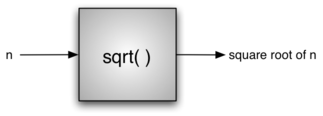
\includegraphics[width=3in]{images/blackbox.png}
\end{figure}
